\section{Distributed Shared Memory}
To speed up computation on a single machine, we use multiple cores to 
run OS threads in parallel. Consider the following example:

\begin{lstlisting}[language=Go]
    for (i := 0; i< n; i++) {
        go work(i,results);
    }  
\end{lstlisting}

\noindent
Here our goal is to run some function \texttt{work} on a perhaps large 
data set of $n$ size. Go easily abstracts this away with the \texttt{go} keyword.\\

\noindent
Now, what if we want to run this on a distributed system?

\begin{lstlisting}[language=Go]
    package main
    import (
        "net/rpc"
    )
    type Args struct{}
    type WorkServer int64
    func (t *WorkServer) DoWork(args *Args, reply *int64) error {
        // Fill reply pointer to send the data back
        work(args.data, *reply);
        return nil
    }
\end{lstlisting}

\noindent
We have to decide now on a system of communication:
\begin{itemize}
    \item How do we interact with sending and receiving data (conflicts, failures, etc.)
    \item How should our coordinator dispatch the work?
    \item What RPCs should we include in our API?
\end{itemize}

\noindent
To solve this problem, we reuse a hardware primitive in the previous Section (\ref{sec:virt}).
\begin{theo}[Multithread Comminucation -- Virtual Memory]

    A multithread process can still communicate between threads by utilizing the same virtual memory space, we call this \textbf{shared memory}.
\end{theo}
\noindent
\underline{\textbf{The goal} is to bring this primitive to the distributed system level.}

\newpage 

\noindent
We clearly define our problem-space:

\begin{Def}[Distributed Shared Memory]
    
    A \textbf{Distributed Shared Memory (DSM)} system is a system that allows multiple processes on different machines to access a shared memory space as if it were local.
    I.e,. create the illusion of a single shared memory across multiple machines to enable multithreaded programs in a distrusted setting.\\

    \noindent
    Applications are built on top of a DSM system who abstracts away consensus and communication. DSM systems 
    connect to the underlying hardware support for shared memory (virtual address translation) to coordinate.
    Page faults are redirected to the DSM system to resolve.\\

    \noindent
    \underline{\textbf{Consensus Model:} Strong consistency, and linearizability.} \textbf{Every} read operation is up-to-date, reflecting the most recent write, if any.

\end{Def}

\noindent
The next solution will be our first draft from which we shall iterate on:
\begin{Def}[DSM -- Page Ownership \& Swap Protocol (Draft)]

    Given a system of $M_i$ machines, the Virtual Address Space (VAS) is evenly divided amongst them. I.e.,
    each machine has some partition of pages it owns. On a local machine, the page table will operate as normal;
    Though, upon a page fault, instead of going to the disk, we redirect to the DSM system. From there we request the missing page
    over the network.
\end{Def}

\begin{figure}[h]
    \centering
    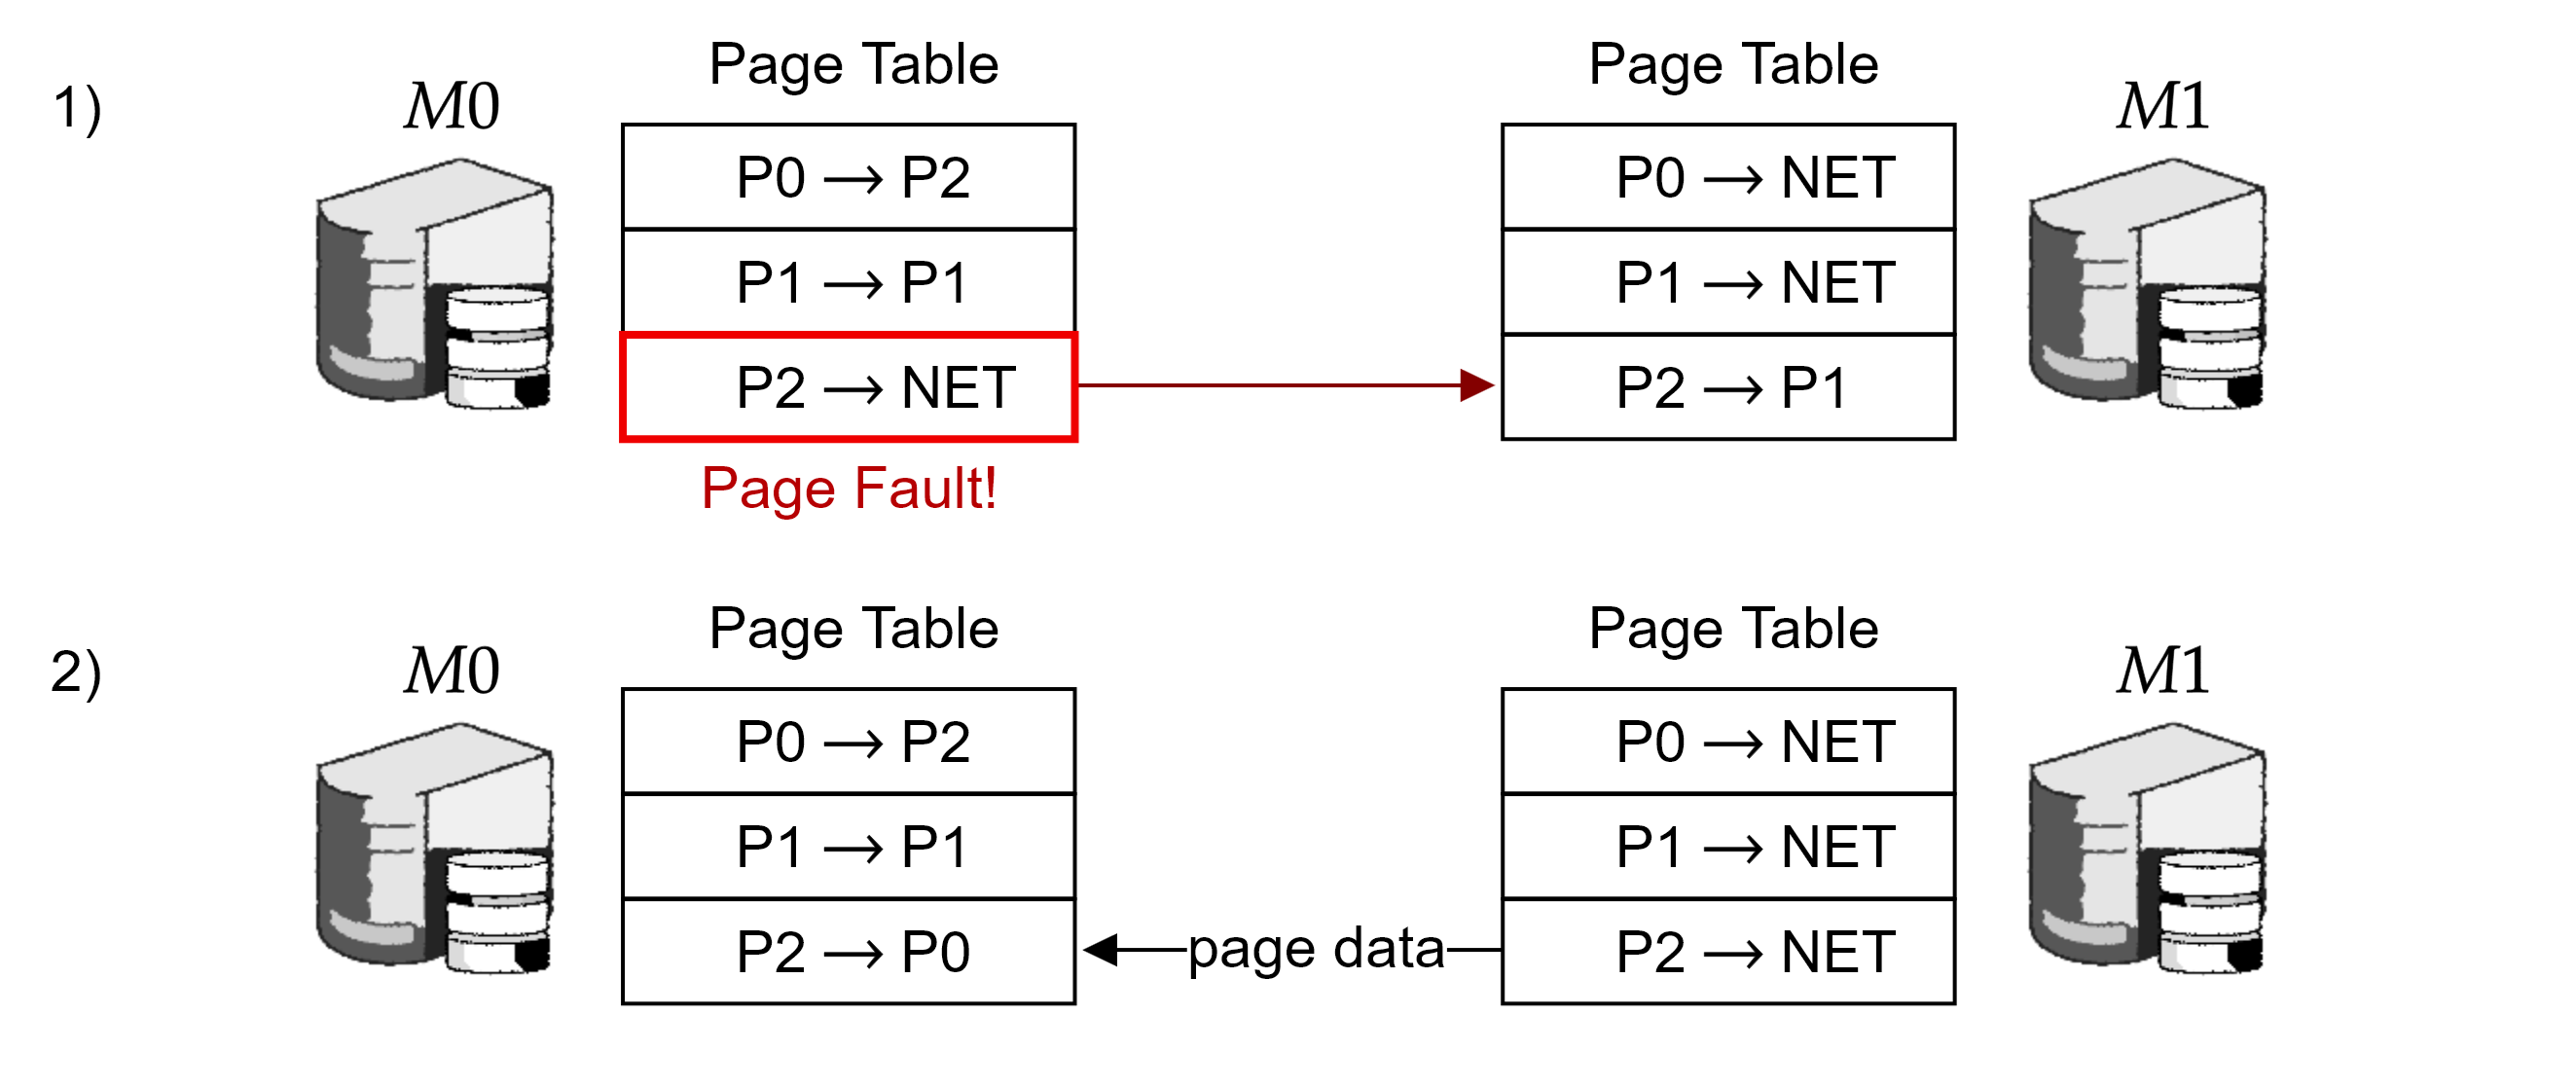
\includegraphics[width=\textwidth]{Sections/shared/share.png}
    \caption{1) System $M_0$ tries to access $P_2$ in virtual memory but incurs a page fault, prompting a request to the DSM system. The DSM resolves that $M_1$ owns the desired page. 
    2) The DSM performs a network swap, sending the actual page data so $M_0$ can load it into physical memory.
    }
    \label{fig:dsm}
\end{figure}

\newpage 

\noindent
Though this is a good start, it's expensive:

\begin{theo}[Sending Pages Over the Network \& False Sharing]

    Pages are often large (4KB), which is expensive to send.
    If two machines $M_0$ and $M_1$ access the same page, but modify different data points (e.g., two different variables),
    the whole page needs to be sent even though the data is not shared. This is called \textbf{false sharing}.
\end{theo}

\noindent
A particular DSM system called \textbf{TreadMarks} solves this problem:
\begin{Def}[TreadMarks -- Page Ownership \& Swap Protocol]

    Given a system of $M_i$ machines, the VAS is evenly divided amongst them.
    When page faults occur, the DSM sends \textbf{diffs} (change history) over the network instead of the entire page.\\

    \noindent
    This allows for all $M_i$ to start with \textbf{RO} (read-only) access on all pages. When $M_j$ wishes to 
    modify a page, $M_j$ notifies all other $M_i$ to invalidate their copies of the page. $M_j$ then gets \textbf{RW} (read-write) access to the page.


    Each write creates a new $V_i$ version of the page ($i$, increases monotonically). Where $V_i$ contains the latest changes, and $V_{i-1}$ a snapshot before the changes.
    
    When $M_i$ page faults, the DSM system requests the page from owner $M_j$, notifying them of the last version $M_i$ saw. The owner $M_j$ locks said page and creates a diff between both $M_i$ and $M_j$'s versions, sending it over the network.
    Both $M_j$ and $M_i$ revert to RO access.\\

    \noindent
    \underline{\textbf{Consensus Model:} Strong consistency, and linearizability.}
\end{Def}

\vspace{-1em}
\begin{figure}[h]
    \centering
    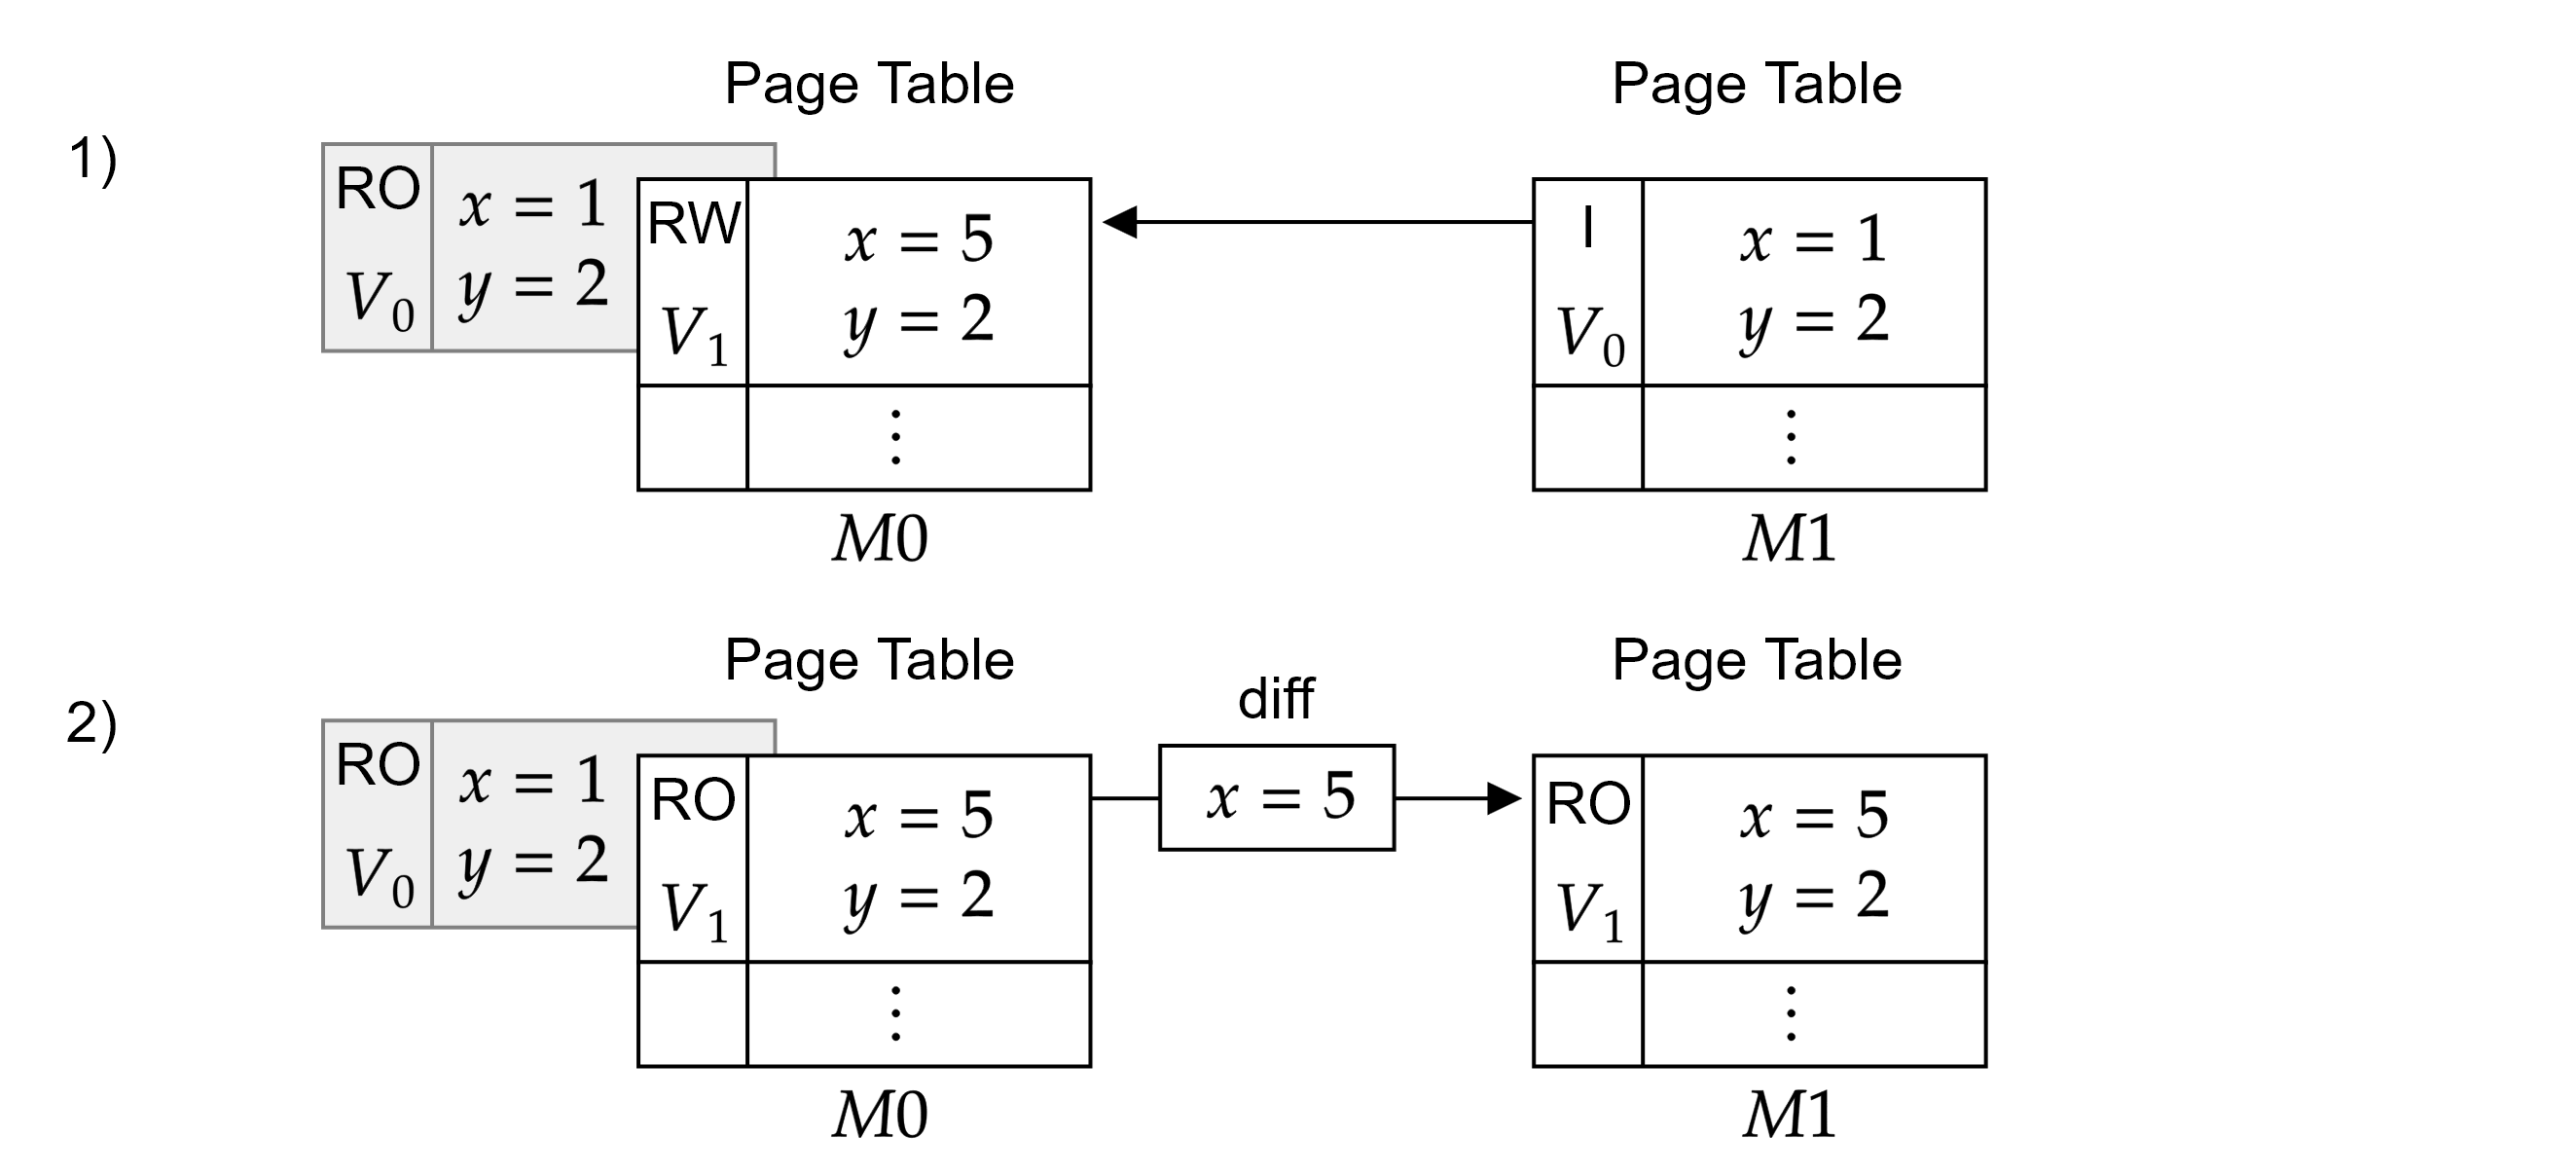
\includegraphics[width=\textwidth]{Sections/shared/tread.png}
    \caption{1) $M1$ requests a page from $M2$. 2) $M2$ sends the diff between $V_0$ and $V_1$ to $M1$.}
    \label{fig:dsm}
\end{figure}

    